% This template has been tested with LLNCS DOCUMENT CLASS -- version 2.20 (10-Mar-2018)

% !TeX spellcheck = en-US
% !TeX encoding = utf8
% !TeX program = pdflatex
% !BIB program = bibtex
% -*- coding:utf-8 mod:LaTeX -*-

% "a4paper" enables:
%  - easy print out on DIN A4 paper size
%
% One can configure a4 vs. letter in the LaTeX installation. So it is configuration dependend, what the paper size will be.
% This option  present, because the current word template offered by Springer is DIN A4.
% We accept that DIN A4 cause WTFs at persons not used to A4 in USA.

% "runningheads" enables:
%  - page number on page 2 onwards
%  - title/authors on even/odd pages
% This is good for other readers to enable proper archiving among other papers and pointing to
% content. Even if the title page states the title, when printed and stored in a folder, when
% blindly opening the folder, one could hit not the title page, but an arbitrary page. Therefore,
% it is good to have title printed on the pages, too.
%
% It is enabled by default as the springer template as of 2018/03/10 uses this as default

% German documents: pass ngerman as class option
 \documentclass[ngerman,runningheads,a4paper]{llncs}[2018/03/10]
% English documents: pass english as class option
%\documentclass[english,runningheads,a4paper]{llncs}[2018/03/10]

%% If you need packages for other papers,
%% START COPYING HERE

% Set English as language and allow to write hyphenated"=words
%
% In case you write German, switch the parameters, so that the command becomes
\usepackage[english,main=ngerman]{babel}
%
% Even though `american`, `english` and `USenglish` are synonyms for babel package (according to https://tex.stackexchange.com/questions/12775/babel-english-american-usenglish), the llncs document class is prepared to avoid the overriding of certain names (such as "Abstract." -> "Abstract" or "Fig." -> "Figure") when using `english`, but not when using the other 2.
% english has to go last to set it as default language
%\usepackage[ngerman,main=english]{babel}
%
% Hint by http://tex.stackexchange.com/a/321066/9075 -> enable "= as dashes
\addto\extrasenglish{\languageshorthands{ngerman}\useshorthands{"}}
%
% Fix by https://tex.stackexchange.com/a/441701/9075
\usepackage{regexpatch}
\makeatletter
\edef\switcht@albion{%
  \relax\unexpanded\expandafter{\switcht@albion}%
}
\xpatchcmd*{\switcht@albion}{ \def}{\def}{}{}
\xpatchcmd{\switcht@albion}{\relax}{}{}{}
\edef\switcht@deutsch{%
  \relax\unexpanded\expandafter{\switcht@deutsch}%
}
\xpatchcmd*{\switcht@deutsch}{ \def}{\def}{}{}
\xpatchcmd{\switcht@deutsch}{\relax}{}{}{}
\edef\switcht@francais{%
  \relax\unexpanded\expandafter{\switcht@francais}%
}
\xpatchcmd*{\switcht@francais}{ \def}{\def}{}{}
\xpatchcmd{\switcht@francais}{\relax}{}{}{}
\makeatother

\usepackage{ifluatex}
\ifluatex
  \usepackage{fontspec}
  \usepackage[english]{selnolig}
\fi

\iftrue % use default-font
  \ifluatex
    % use the better (sharper, ...) Latin Modern variant of Computer Modern
    \setmainfont{Latin Modern Roman}
    \setsansfont{Latin Modern Sans}
    \setmonofont{Latin Modern Mono} % "variable=false"
    %\setmonofont{Latin Modern Mono Prop} % "variable=true"
  \else
    % better font, similar to the default springer font
    % cfr-lm is preferred over lmodern. Reasoning at http://tex.stackexchange.com/a/247543/9075
    \usepackage[%
      rm={oldstyle=false,proportional=true},%
      sf={oldstyle=false,proportional=true},%
      tt={oldstyle=false,proportional=true,variable=false},%
      qt=false%
    ]{cfr-lm}
  \fi
\else
  % In case more space is needed, it is accepted to use Times New Roman
  \ifluatex
    \setmainfont{TeX Gyre Termes}
    \setsansfont[Scale=.9]{TeX Gyre Heros}
    % newtxtt looks good with times, but no equivalent for lualatex found,
    % therefore tried to replace with inconsolata.
    % However, inconsolata does not look good in the context of LNCS ...
    %\setmonofont[StylisticSet={1,3},Scale=.9]{inconsolata}
    % ... thus, we use the good old Latin Modern Mono font for source code.
    \setmonofont{Latin Modern Mono} % "variable=false"
    %\setmonofont{Latin Modern Mono Prop} % "variable=true"
  \else
    % overwrite cmodern with the Times variant
    \usepackage{newtxtext}
    \usepackage{newtxmath}
    \usepackage[zerostyle=b,scaled=.9]{newtxtt}
  \fi
\fi

\ifluatex
\else
  % fontenc and inputenc are not required when using lualatex
  \usepackage[T1]{fontenc}
  \usepackage[utf8]{inputenc} %support umlauts in the input
\fi

\usepackage{graphicx}

% backticks (`) are rendered as such in verbatim environment. See https://tex.stackexchange.com/a/341057/9075 for details.
\usepackage{upquote}

% Nicer tables (\toprule, \midrule, \bottomrule - see example)
\usepackage{booktabs}

%extended enumerate, such as \begin{compactenum}
\usepackage{paralist}

%put figures inside a text
%\usepackage{picins}
%use
%\piccaptioninside
%\piccaption{...}
%\parpic[r]{\includegraphics ...}
%Text...

% For easy quotations: \enquote{text}
% This package is very smart when nesting is applied, otherwise textcmds (see below) provides a shorter command
\usepackage{csquotes}

% For even easier quotations: \qq{text}
\usepackage{textcmds}

%enable margin kerning
\RequirePackage[%
  babel,%
  final,%
  expansion=alltext,%
  protrusion=alltext-nott]{microtype}%
% \texttt{test -- test} keeps the "--" as "--" (and does not convert it to an en dash)
\DisableLigatures{encoding = T1, family = tt* }

%tweak \url{...}
\usepackage{url}
%\urlstyle{same}
%improve wrapping of URLs - hint by http://tex.stackexchange.com/a/10419/9075
\makeatletter
\g@addto@macro{\UrlBreaks}{\UrlOrds}
\makeatother
%nicer // - solution by http://tex.stackexchange.com/a/98470/9075
%DO NOT ACTIVATE -> prevents line breaks
%\makeatletter
%\def\Url@twoslashes{\mathchar`\/\@ifnextchar/{\kern-.2em}{}}
%\g@addto@macro\UrlSpecials{\do\/{\Url@twoslashes}}
%\makeatother

% Diagonal lines in a table - http://tex.stackexchange.com/questions/17745/diagonal-lines-in-table-cell
% Slashbox is not available in texlive (due to licensing) and also gives bad results. This, we use diagbox
%\usepackage{diagbox}

% Required for package pdfcomment later
\usepackage{xcolor}

% For listings
\usepackage{listings}
\lstset{%
  basicstyle=\ttfamily,%
  columns=fixed,%
  basewidth=.5em,%
  xleftmargin=0.5cm,%
  captionpos=b}%
\renewcommand{\lstlistingname}{List.}
% Fix counter as described at https://tex.stackexchange.com/a/28334/9075
\usepackage{chngcntr}
\AtBeginDocument{\counterwithout{lstlisting}{section}}

% Enable nice comments
\usepackage{pdfcomment}
%
\newcommand{\commentontext}[2]{\colorbox{yellow!60}{#1}\pdfcomment[color={0.234 0.867 0.211},hoffset=-6pt,voffset=10pt,opacity=0.5]{#2}}
\newcommand{\commentatside}[1]{\pdfcomment[color={0.045 0.278 0.643},icon=Note]{#1}}
%
% Compatibality with packages todo, easy-todo, todonotes
\newcommand{\todo}[1]{\commentatside{#1}}
% Compatiblity with package fixmetodonotes
\newcommand{\TODO}[1]{\commentatside{#1}}

% Bibliopgraphy enhancements
%  - enable \cite[prenote][]{ref}
%  - enable \cite{ref1,ref2}
% Alternative: \usepackage{cite}, which enables \cite{ref1, ref2} only (otherwise: Error message: "White space in argument")

% Doc: http://texdoc.net/natbib
\usepackage[%
  square,        % for square brackets
  comma,         % use commas as separators
  numbers,       % for numerical citations;
%  sort,          % orders multiple citations into the sequence in which they appear in the list of references;
  sort&compress, % as sort but in addition multiple numerical citations
                 % are compressed if possible (as 3-6, 15);
]{natbib}
% In the bibliography, references have to be formatted as 1., 2., ... not [1], [2], ...
\renewcommand{\bibnumfmt}[1]{#1.}

\ifluatex
  % does not work when using luatex
  % see: https://tex.stackexchange.com/q/419288/9075
\else
  % Prepare more space-saving rendering of the bibliography
  % Source: https://tex.stackexchange.com/a/280936/9075
  \SetExpansion
  [ context = sloppy,
    stretch = 30,
    shrink = 60,
    step = 5 ]
  { encoding = {OT1,T1,TS1} }
  { }
\fi

% Put footnotes below floats
% Source: https://tex.stackexchange.com/a/32993/9075
\usepackage{stfloats}
\fnbelowfloat

% Enable that parameters of \cref{}, \ref{}, \cite{}, ... are linked so that a reader can click on the number an jump to the target in the document
\usepackage{hyperref}
% Enable hyperref without colors and without bookmarks
\hypersetup{hidelinks,
  colorlinks=true,
  allcolors=black,
  pdfstartview=Fit,
  breaklinks=true}
%
% Enable correct jumping to figures when referencing
\usepackage[all]{hypcap}

\usepackage[group-four-digits,per-mode=fraction]{siunitx}

%enable \cref{...} and \Cref{...} instead of \ref: Type of reference included in the link
\usepackage[capitalise,nameinlink]{cleveref}
%Nice formats for \cref
\usepackage{iflang}
\IfLanguageName{ngerman}{
  \crefname{table}{Tab.}{Tab.}
  \Crefname{table}{Tabelle}{Tabellen}
  \crefname{figure}{\figurename}{\figurename}
  \Crefname{figure}{Abbildung}{Abbildungen}
  \crefname{equation}{Gleichung}{Gleichungen}
  \Crefname{equation}{Gleichung}{Gleichungen}
  \crefname{listing}{\lstlistingname}{\lstlistingname}
  \Crefname{listing}{Listing}{Listings}
  \crefname{section}{Abschnitt}{Abschnitte}
  \Crefname{section}{Abschnitt}{Abschnitte}
  \crefname{paragraph}{Abschnitt}{Abschnitte}
  \Crefname{paragraph}{Abschnitt}{Abschnitte}
  \crefname{subparagraph}{Abschnitt}{Abschnitte}
  \Crefname{subparagraph}{Abschnitt}{Abschnitte}
}{
  \crefname{section}{Sect.}{Sect.}
  \Crefname{section}{Section}{Sections}
  \crefname{listing}{\lstlistingname}{\lstlistingname}
  \Crefname{listing}{Listing}{Listings}
}


%Intermediate solution for hyperlinked refs. See https://tex.stackexchange.com/q/132420/9075 for more information.
\newcommand{\Vlabel}[1]{\label[line]{#1}\hypertarget{#1}{}}
\newcommand{\lref}[1]{\hyperlink{#1}{\FancyVerbLineautorefname~\ref*{#1}}}

\usepackage{xspace}
%\newcommand{\eg}{e.\,g.\xspace}
%\newcommand{\ie}{i.\,e.\xspace}
\newcommand{\eg}{e.\,g.,\ }
\newcommand{\ie}{i.\,e.,\ }

%introduce \powerset - hint by http://matheplanet.com/matheplanet/nuke/html/viewtopic.php?topic=136492&post_id=997377
\DeclareFontFamily{U}{MnSymbolC}{}
\DeclareSymbolFont{MnSyC}{U}{MnSymbolC}{m}{n}
\DeclareFontShape{U}{MnSymbolC}{m}{n}{
  <-6>    MnSymbolC5
  <6-7>   MnSymbolC6
  <7-8>   MnSymbolC7
  <8-9>   MnSymbolC8
  <9-10>  MnSymbolC9
  <10-12> MnSymbolC10
  <12->   MnSymbolC12%
}{}
\DeclareMathSymbol{\powerset}{\mathord}{MnSyC}{180}

\ifluatex
\else
  % Enable copy and paste - also of numbers
  % This has to be done instead of \usepackage{cmap}, because it does not work together with cfr-lm.
  % See: https://tex.stackexchange.com/a/430599/9075
  \input glyphtounicode
  \pdfgentounicode=1
\fi

% correct bad hyphenation here
\hyphenation{op-tical net-works semi-conduc-tor}

%% END COPYING HERE


% Add copyright
% Do that for the final version or if you send it to colleagues
\iffalse
  %state: intended|submitted|llncs
  %you can add "crop" if the paper should be cropped to the format Springer is publishing
  \usepackage[intended]{llncsconf}

  \conference{name of the conference}

  %in case of "llncs" (final version!)
  %example: llncs{Anonymous et al. (eds). \emph{Proceedings of the International Conference on \LaTeX-Hacks}, LNCS~42. Some Publisher, 2016.}{0042}
  \llncs{book editors and title}{0042} %% 0042 is the start page
\fi

% For demonstration purposes only
\usepackage[math]{blindtext}
\usepackage{mwe}


\begin{document}

\title{Mining und Einigkeit in Bitcoin}
%If Title is too long, use \titlerunning
%\titlerunning{Short Title}

%Single insitute
\author{Nico Daßler}
%If there are too many authors, use \authorrunning
%\authorrunning{First Author et al.}
\institute{Friedrich-Alexander Universität Erlangen-Nürnberg}

%% Multiple insitutes - ALTERNATIVE to the above
% \author{%
%     Firstname Lastname\inst{1} \and
%     Firstname Lastname\inst{2}
% }
%
%If there are too many authors, use \authorrunning
%  \authorrunning{First Author et al.}
%
%  \institute{
%      Insitute 1\\
%      \email{...}\and
%      Insitute 2\\
%      \email{...}
%}

\maketitle

\begin{abstract}
  \todo{place proper abstract here} 
  \lipsum[1]
\end{abstract}

\begin{keywords}
  bitcoin, mining, einigung, verteilt
\end{keywords}

\section{Einführung}\label{sec:einführung}

Ideen:

Jede Art von Währung muss dem Betrug mit dieser Währung entgegenwirken. Bei gedrucktem Geld zum Beispiel muss verhindert werden, dass Falschgeld hergestellt werden kann. Dies wird durch spezielle Sicherheitsmerkmale auf Geldscheinen erreicht, welche den Nachdruck unmöglich machen sollen. Bei digitalen Währungen gibt es ähnliche Probleme. Zum Beispiel muss verifiziert werden, dass bei einer Transaktion kein kopiertes Geld zum Einsatz kommt. Dazu gehört das sogenannte \textit{double spend} Problem, bei dem ein bestimmter Betrag mehrfach ausgegeben werden könnte...

\section{Grundlagen}\label{sec:grundlagen}

Erklärung wie Blöcke aufgebaut sind, was Blöcke enthalten, verschiedene Bausteine des Bitcoin Netzwerks.

\subsection{Transaktion}\label{sec:transaktionen}

Um mit Bitcoin Transaktionen durchzuführen wird mithilfe eines sogenannten Wallets (dt. Geldbeutel) eine Transaktion durchgeführt. Die Wallet Software speichert die privaten und öffentlichen Schlüssel, die zur Signatur von Transaktionen und zur Verifikation des Besitzes der Bitcoins eingesetzt werden. Außerdem bildet die Wallet Software eine syntaktisch korrekte Transaktion und speist diese in das Bitcoin Netzwerk ein. Die für die nachfolgenden Abschnitte wichtigen Datenfelder und Mechanismen einer Transaktion werden in diesem Abschnitt beschrieben.

Digitale Signaturen werden eingesetzt um zu beweisen, dass ein beliebiger Datenstrom (z.B. eine E-Mail) tatsächlich von einer bestimmten Person verfasst wurde. Dabei wird mithilfe des Datenstroms und des privaten Schlüssels eine Signatur berechnet, welche dann mithilfe des öffentlichen Schlüssels verifziert werden kann. Mithilfe des Datenstroms, des öffentlichen Schlüssels und der Signatur, kann jeder sicherstellen, dass der Datenstrom vom Besitzer des privaten Schlüssels verfasst wurde. In Bitcoin wird der \textit{Elliptic Curve Digital Signature Algorithm} eingesetzt um den Besitz von Bitcoin zu beweisen \citep{bitcoinbook}.

In Bitcoin ist die Nachricht, die signiert wird, die Trasaktion. Dabei können Teile oder die gesamte Transaktion in der Signatur verwendet werden. Das ist in verschiedenen Szenarien nützlich \citep{bitcoinbook}. Mithilfe von Signaturen und deren Verifikationen werden unteilbare Geldmittel (engl. \textit{funds}) \textit{unlocked} bzw. für die Nutzung in einer weiteren Transaktion freigeschaltet. Diese Geldmittel werden \textit{UTXOs} genannt. UTXO steht für einen \textit{unspent transaction output} \citep{bitcoinbook}, also ein Geldmittel, dass noch nicht ausgegeben wurde . Das Freischalten und Sperren wird in Form von Skripten innerhalb einer Transaktion spezifiziert. 

\begin{figure}
  \centering
  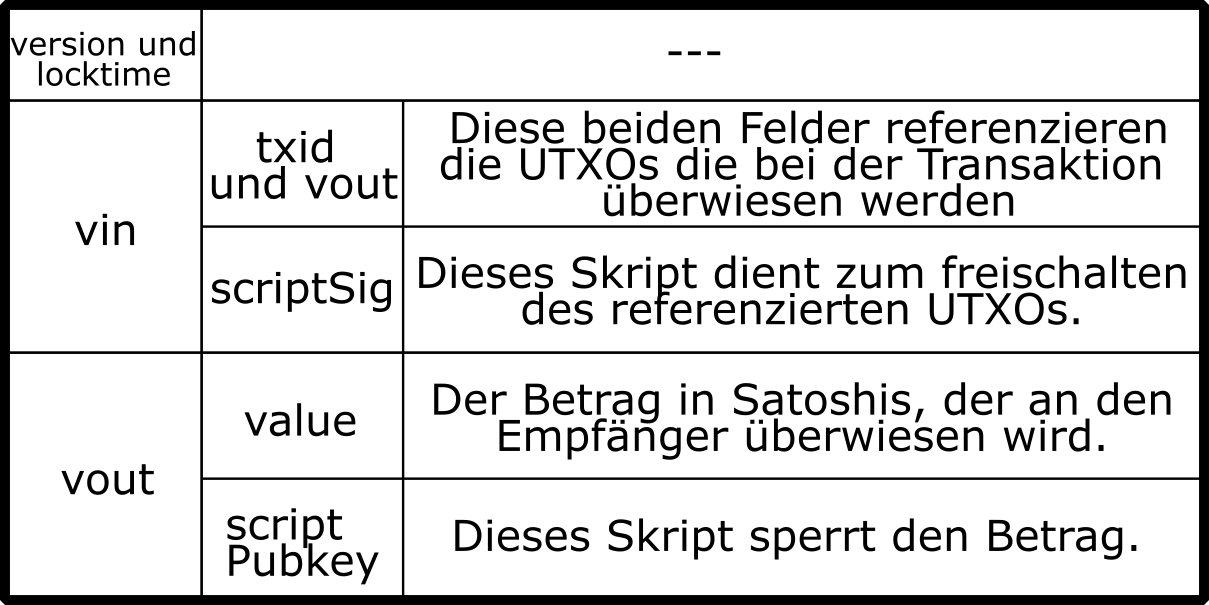
\includegraphics[width=.8\textwidth]{grafiken/tableTransaction.png}
  \caption{Zeigt die für diese Arbeit relevanten Felder einer Transaktion.}
  \label{fig:transactionTable}
\end{figure}

\Cref{fig:transactionTable} zeigt den Aufbau einer Transaktion. Das Feld \textit{vout} beschreibt die neuen UTXOs (eine Liste), die bei der Transaktion angelegt werden. Jeder dieser UTXOs hat einen Betrag und ein Skript mit dem der Betrag freigeschaltet werden kann. Das Skript ist in der Sprache \textit{Script} geschrieben. Script ist eine "Forth-like reverse-polish notation stack-based execution language" \citep{bitcoinbook} und wird an dieser Stelle nicht im Detail beschrieben. Wichtig ist jedoch, dass mit diesen Skripten Signaturen erzeugt und geprüft werden können. In den meisten Fällen wird der UTXO mit dem \textit{Pay-to-Public-Key-Hash} \citep{bitcoinbook} Skript gesperrt. Das bedeutet, dass zum Entsperren eine Signatur über die Transaktion benötigt wird und ein öffentlicher Schlüssel dessen Hash Wert mit dem im Skript gegebenen \textit{Public Key Hash} übereinstimmen muss. Im Feld \textit{vin} werden die Geldmittel spezifziert, die versendet werden. Dies passiert über die Referenz auf UTXOs, die nach dem oben beschriebenen Verfahren entsprerrt werden müssen.

Auf diese Weise entsteht eine Verkettung von Transaktionen. Die UTXOs einer Transaktionen dienen als Geldmittel für eine andere Transaktion, welche wieder neue UTXOs anlegt, welche wieder als Geldmittel verwendet werden können. Die UTXOs sind dabei unteilbar. Soll zum Beispiel eine Transaktion über 5 Bitcoin durchgeführt werden und es steht nur ein UTXO in Höhe von 10 Bitcoin zur Verfügung \footnote{Der Betrag eines UTXOs wird nur einmal im vout Feld einer Transaktion spezifiziert. Im vin ist der Betrag implizit über die Referenz auf den UTXO enthalten.} so muss der Sender zwei UTXOs im vout Feld definieren. Einen für den Empfänger der 5 Bitcoin und einen für sich selbst als Wechselgeld.

Bei jeder Transaktion werden außerdem Gebühren durch den Sender definiert. Diese Gebühren sind nicht notwendig allerdings beschleunigen sie die Verifizierung der Transaktion und spielen eine wichtige Rolle beim Mining. Die Gebühren werden über die Differenz der vin und der vout Beträge implizit angegeben.

\subsection{Block}\label{sec:block}

Die im letzten Abschnitt beschriebenen Transaktionen werden in sogenannte Blöcke aggregiert um innerhalb des Bitcoin Netzwerks ein gemeinsames Verständnis zu schaffen, welche UTXOs existieren und welche bereits ausgegeben wurden. Ein Block beginnt mit einigen Metadaten und dem \textit{Block Header}. Der Block Header enthält einige für das Mining relevante Felder, welche im Folgenden erklärt werden.

\begin{figure}
  \centering
  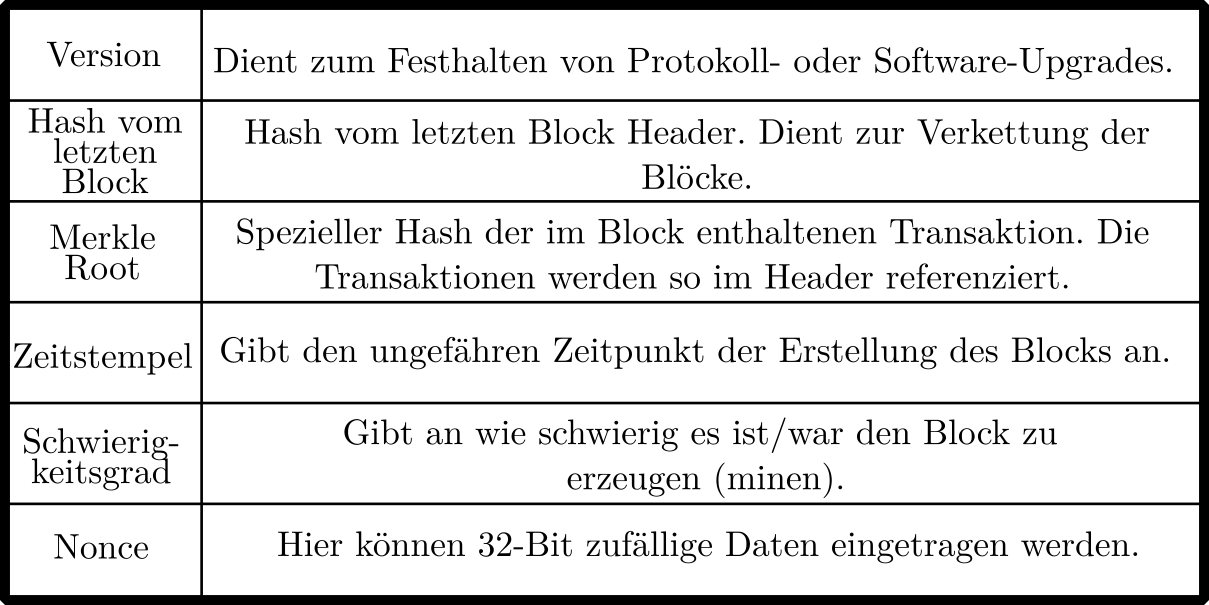
\includegraphics[width=.8\textwidth]{grafiken/tableBlock.png}
  \caption{Zeigt den Aufbau des Block Headers.}
  \label{fig:blockTable}
\end{figure}

\Cref{fig:blockTable} zeigt den Aufbau des Block Headers. Der Hash vom letzten Block (bzw. vom letzten Block Header) ist eines der wichtigsten Elemente im Block. Er sorgt dafür, dass Blöcke miteinander verknüpft sind. Die Blöcke formen damit eine Kette von Blöcken welche als Blockchain bezeichnet wird. Die Merkle Root ist eine Zusammenfassung der im Block enthaltenen Transaktionen \citep{bitcoinbook}. Sie stellt sicher, dass eine Veränderung der Transaktionen eine Veränderung des Headers zur Folge hat. Der Schwierigkeitsgrad und die Nonce werden bei der Erstellung (Mining) eines Blocks verwendet. Um einen gültigen Block zu erzeugen muss der Hash des Headers kleiner sein als der Schwierigkeitsgrad (auch \textit{Difficulty Target} genannt) der im Header spezifiziert wird. Da das Ergebnis einer Hash Funktion nicht vorhergesagt werden kann müssen verschiedenen Header ausprobiert werden. Das Nonce Feld im Header dient zur Veränderung des Headers und damit zur Veränderung des Hash Wertes. Andere Felder dürfen nicht verändert werden, da der Header sonst nicht mehr gültig ist. Um das Target zu unterschreiten, muss Rechenleistung aufgebracht werden (ausprobieren vieler verschiedener Nonce Werte). Das diese Leistung tatsächlich erbracht wurde kann mit einem einzelnen Durchlauf durch die Hash Funktion verifiziert werden. Dieser Vorgang wird \textit{Proof-of-Work} genannt.

\subsection{Betrug in Bitcoin}\label{sec:betrug}

Mit den in \Cref{sec:transaktionen} besprochenenen Mechanismen kann ein Empfänger von Bitcoins bestätigen, dass der Absender der tatsächliche Besitzer der Bitcoins ist. Der Empfänger kann die Signaturen verifizieren um die Kette des Besitzes zurückzuverfolgen \citep{bitcoinPDF}. Es ist also nicht möglich Bitcoins zu kopieren oder zu erzeugen, da die Bitcoins bis zu ihrem Ursprung zurückverfolgt werden können. Die Transaktionen werden dabei in der Blockchain gespeichert (siehe \Cref{sec:block}). Dabei stellt sich die Frage wie in einem verteilten System Einigkeit über den Zustand der Blockchain entstehen kann und wie diese gegen Veränderung geschützt wird. Wäre es möglich eine Transaktion im nachhinein zu verändern, so könnte ein Käufer die selben Bitcoins mehrfach ausgegeben. In den nachfolgenden Abschnitten wird dieses Problem (das \textit{Double-Spend Problem}) durch Mining und das Befolgen einiger einfachen Regeln bei jedem Netzwerkknoten gelöst.


\section{Informationsverbreitung}\label{sec:informationsverbreitung}

In den folgenden beiden Abschnitten werden die Regeln beschrieben, mit denen Transaktionen und Blöcke vom Bitcoin Netzwerk akzeptiert und verteilt werden. Das Netzwerk ist ein \textit{Peer-to-Peer Netzwerk}. Obwohl die Knoten in einem P2P Netzwerk gleichgestellt sind, nehmen sie unterschiedliche Aufgaben wahr \citep{bitcoinbook}. Nachfolgend werden Knoten, die Routing Aufgaben übernehmen und eine komplette Kopie der Blockchain enthalten als \textit{Full Nodes} bezeichnet. Als Wallet werden Knoten bezeichnet, die lediglich die Schlüssel eines Nutzers verwalten und sich an Full Nodes wenden um Zugriff auf die Blockchain zu erhalten. In \Cref{sec:mining} wird zusätzlich der Begriff \textit{Miner} für Knoten verwendet die Mining durchführen. \Cref{fig:basicNetwork} zeigt ein Teil dieser Komponenten in einem einfachen Bitcoin Netzwerk. 

% TODO: This should not be in the document before section Informationsverbreitung
\begin{figure}
  \centering
  \frame{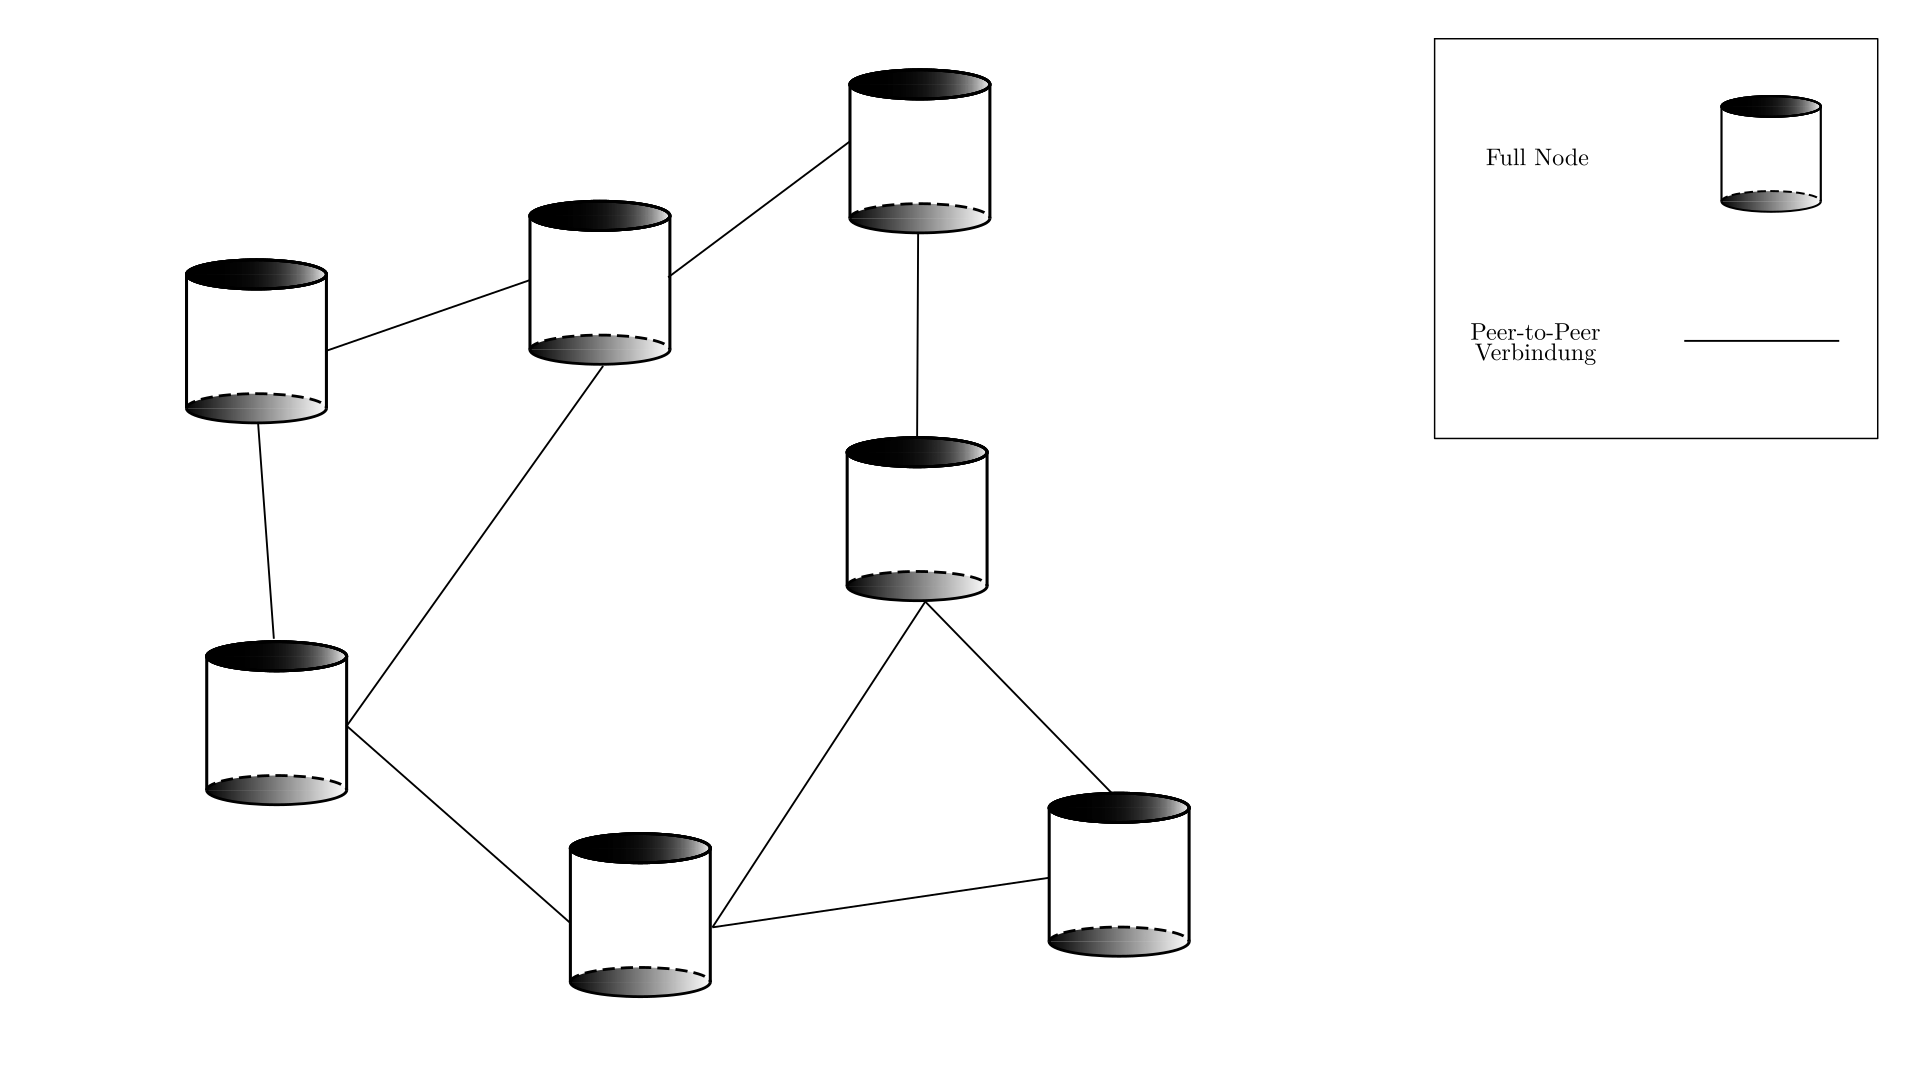
\includegraphics[width=.8\textwidth]{grafiken/network.png}}
  \caption{Der Aufbau eines einfachen Bitcoin Netzwerks mit Peer-to-Peer Verbindungen und Full Nodes.}
  \label{fig:basicNetwork}
\end{figure}

\subsection{Verbreitung von Transaktionen}\label{sec:transaktionsverbreitung}

Eine Transaktion wird typischerweise in einem Wallet-Knoten erzeugt. Zum Beispiel wenn ein Nutzer einen anderen für einen Service oder ein Produkt bezahlen möchte. Die Transaktion wird entsprechend der in \Cref{sec:transaktionen} beschriebenen Struktur aufgebaut und anschließend über eine Full Node an das P2P Netzwerk übergeben. Beim Erhalt einer Transaktion wird dessen Struktur und Inhalt überprüft. Falls alle Kriterien erfüllt sind, wird die Transaktion an benachbarte Knoten weitergegeben und in den lokalen Speicher für unbestätigte Transaktionen übertragen (auch \textit{Memory Pool} oder \textit{Transaction Pool} genannt). In \Cref{fig:transactionPropagation} wird dieser Vorgang mit einer einzelnen Transaktion dargestellt. Die Transaktion wird in vereinfachter Form nur über die ID (txid) dargestellt, die normalerweise 256-Bit lang ist.

\begin{figure}
  \centering
  \frame{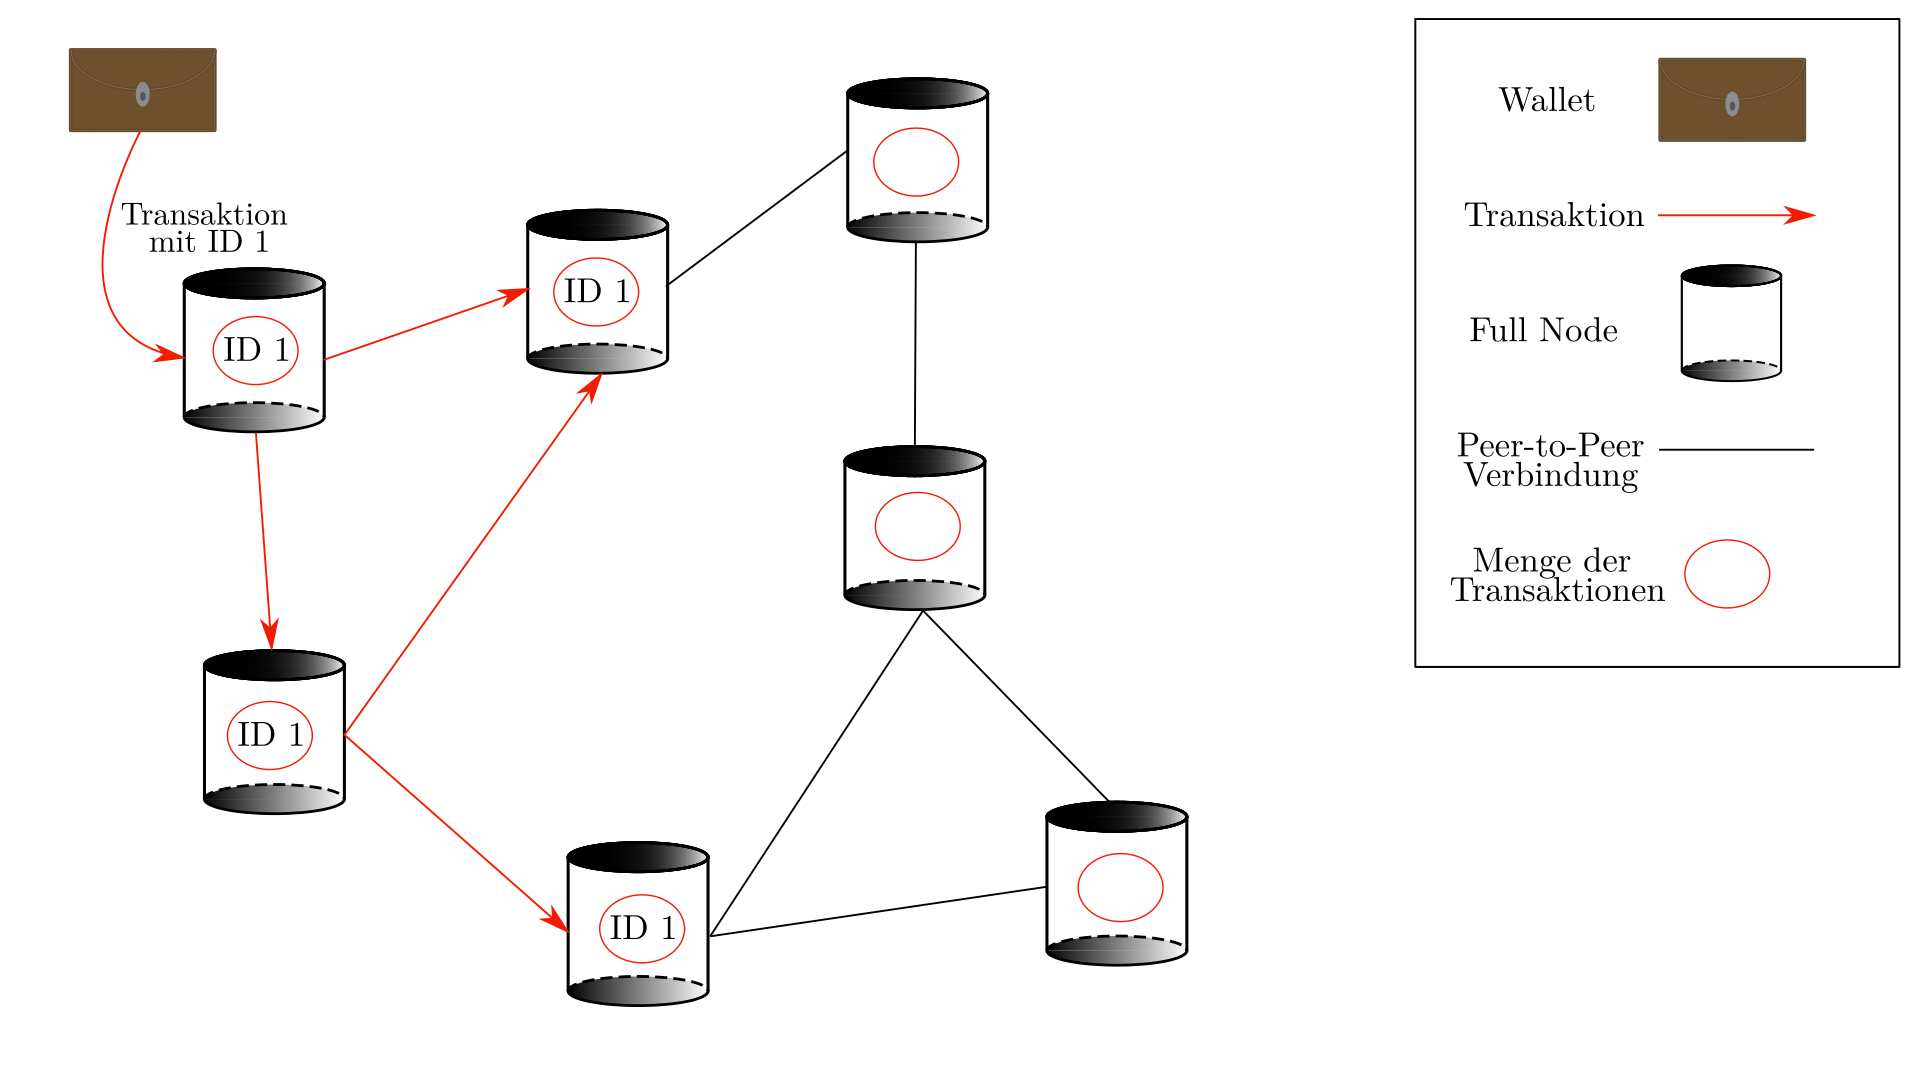
\includegraphics[width=.8\textwidth]{grafiken/transactionPropagation.png}}
  \caption{Die Verbreitung einer Transaktion im P2P Netzwerk. Nach der Überprüfung einer Transaktion wird diese im Memory Pool gespeichert und an benachbarte Knoten weitergeleitet.}
  \label{fig:transactionPropagation}
\end{figure}

Um zu Bestätigen, dass eine Transaktion gültig ist wird zunächst geprüft ob der Aufbau korrekt ist. Danach werden einige formale Aspekte des Inhalts überprüft wie zum Beispiel ob die Maximallänge überschritten wurde oder die vin und vout Listen beide mindestens ein Element haben. Weitere wichtige Kriterien\footnote{Es gibt weitere Kriterien, die allerdings weniger relevant für das Verständnis des Minings und der Konsensfindung sind. Diese Regeln sind in \citep{bitcoinbook} oder im Bitcoin Source Code \citep{bitcoincore} aufgelistet.} sind:

\begin{itemize}

\item Die txids von allen vin Elementen müssen im Transaction Pool oder in einem Block der Blockchain\footnote{Für schnelleren Zugriff werden diese im UTXO Set abgespeichert.} enthalten sein. Falls keine passende Transaktion für eines der Elemente gefunden wird, wird die Transaktion dem \textit{Orphan Transaction Pool} hinzugefügt.

\item Keiner der Inputs darf in einer anderen Transaktion als Input vorkommen, da er sonst bereits ausgegeben wurde. Das gilt auch für Transaktionen mit dem gleichen Input im Orphan Transaction Pool.

\item Die Skripte zum Sperren und Entsperren für jedes Input und Output Paar müssen ein gültiges Ergebnis liefern.

\end{itemize}

Wird eine der oben genannten Regeln nicht eingehalten wird diese Transaktion verworfen und nicht im Netzwerk verbreitet. Alle ehrlichen Full Nodes verhindern somit die Verbreitung von falschen oder betrügerischen Transaktionen. Es werden zum Beispiel Transaktionen aussortiert, deren Ersteller nicht Besitzer der UTXOs ist oder wenn eine Transaktion versucht einen UTXO zweimal auszugeben. Durch diese einfachen Regeln entsteht damit ein Konsens im Netzwerk welche Transaktionen gültig sind und welche nicht. Allerdings können doppelt ausgegebene UTXOs nur mithilfe der Blockchain aussortiert werden. Im nächsten Abschnitt wird eine weitere Menge von Regeln beschrieben, die im Netzwerk Konsens über den Zustand der Blockchain erreichen.

\subsection{Verbreitung von Blöcken}\label{sec:blockverbreitung}

Nachdem ein Block von einem Mining Knoten erstellt wurde (siehe \Cref{sec:mining}), wird dieser an das Netzwerk übergeben. Ähnlich wie bei der Verbreitung von Transaktionen wird eine Menge von Regeln für jeden Block überprüft. Wird eine der Regeln verletzt, wird der Block verworfen. Der Block muss die in \Cref{sec:block} beschriebene Struktur aufweisen. Außerdem muss der Hash des Headers kleiner sein als das angegebene \textit{Difficulty Target} und alle enthaltenen Transaktionen müssen die in \Cref{sec:transaktionsverbreitung} aufgeführten Regeln einhalten. Durch diese Regeln wird sichergestellt, dass keiner der Miner betrügt. Versucht ein Miner zum Beispiel falsche Transaktionen in einen Block einzubauen, wird der Block vom Netzwerk abgelehnt und der Miner erhält dadurch keinen Gewinn für die aufgewendeten Kosten.

Wenn eine Full Node einen Block erhält, der die Regeln einhält wird er versuchen diesen an die Blockchain anzuhängen. Dafür muss der Knoten herausfinden welcher Block in der Blockchain der Vorgänger des neuen Knotens ist. Das Headerfeld Hash vom letzten Block wird dafür mit den letzten Blöcken der Blockchain verglichen. Dabei kann es zu drei Fällen kommen (siehe auch \Cref{blockchainTypes}):

\begin{itemize}

\item Der passende Block ist das Ende (der neueste Block) der bestehenden Blockchain. Der Block wird an diese Blockchain, die auch \textit{Main Chain} genannt wird, angehängt.

\item Der passende Block ist nicht das Ende der Blockchain sondern ein Block weiter vorne. Auch dieser Fall ist für das Bitcoin Protokoll normal und der Block wird angehängt und bildet eine sogenannte \textit{Secondary Chain}.

\item Der passende Block konnte nicht gefunden werden. Der Block wird im sogenannten Orphan Block Pool gespeichert bis der Elternblock empfangen wird und beide der Blockchain hinzugefügt werden können.

\end{itemize}

\begin{figure}
  \centering
  \frame{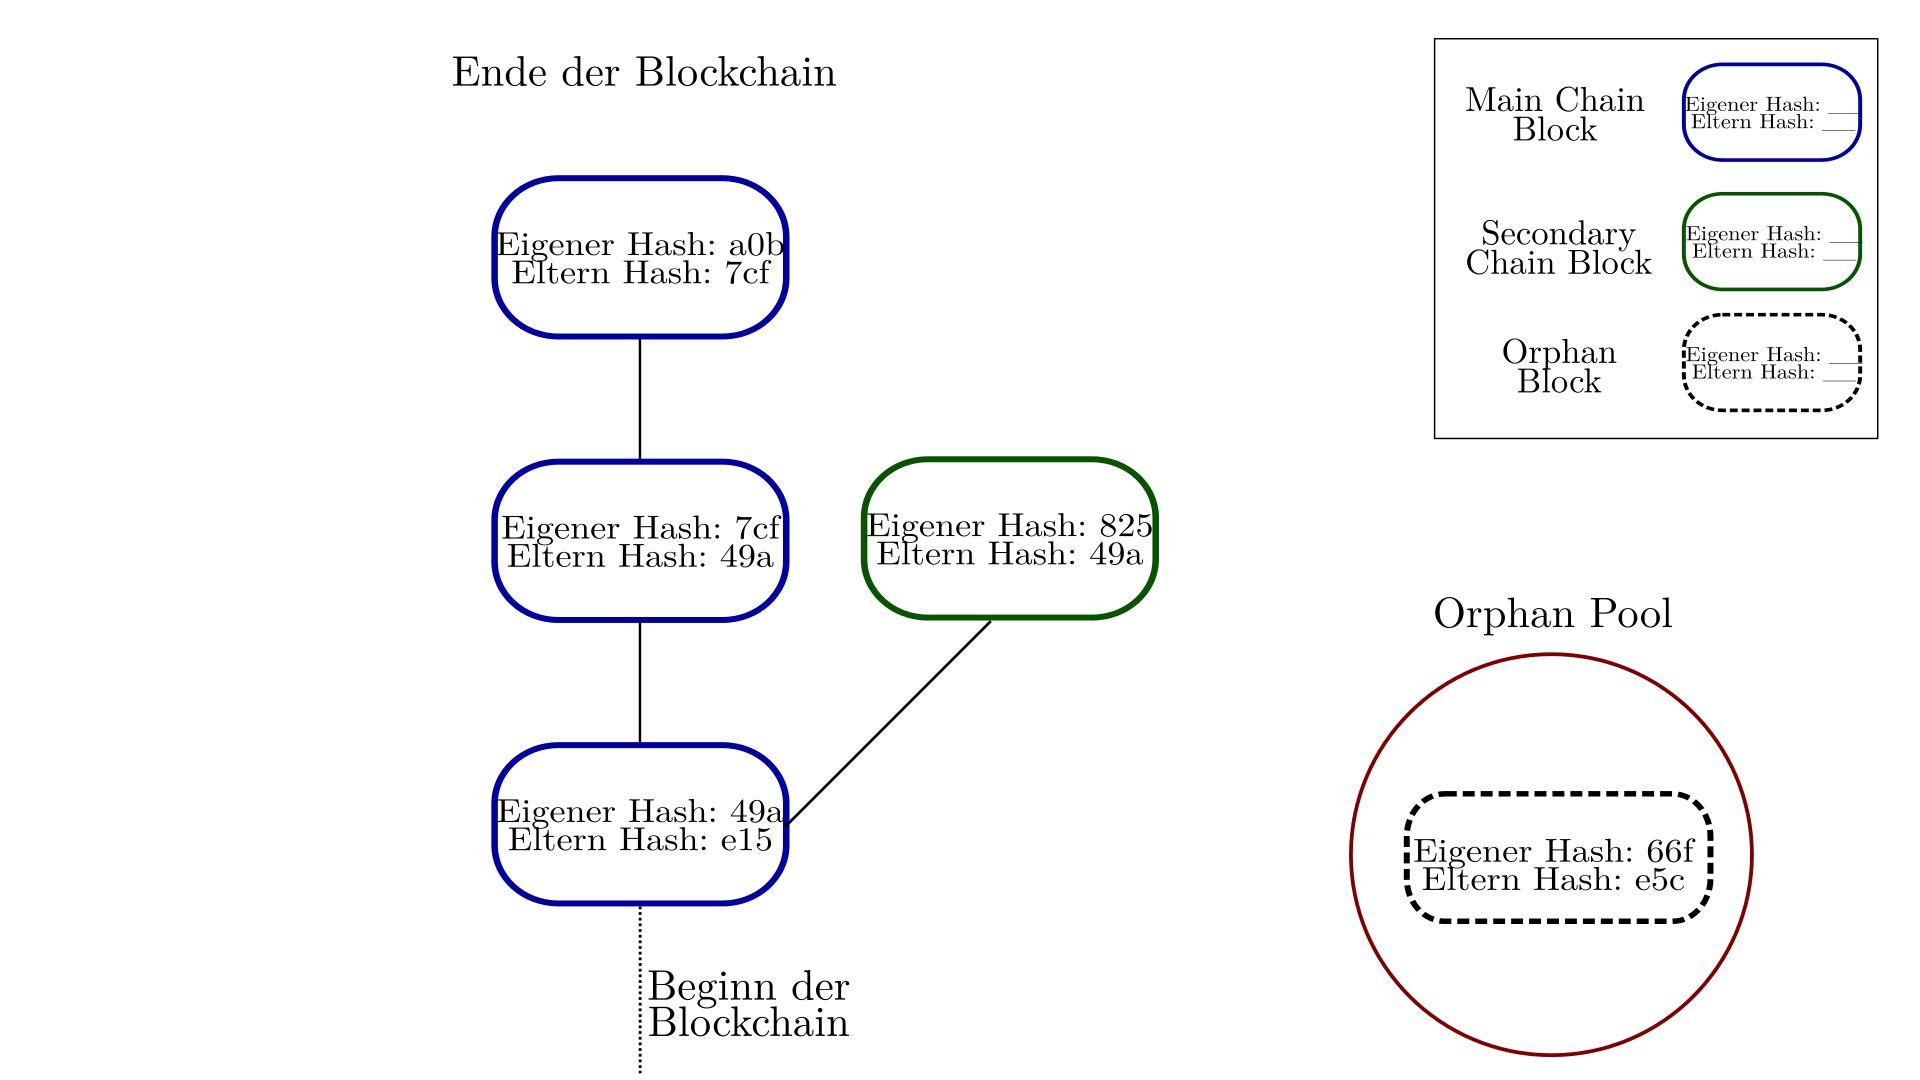
\includegraphics[width=.8\textwidth]{grafiken/blockchainTypes.png}}
  \caption{Die verschiedenen Typen von Blockchains: Main Chain, Secondary Chain und Orphan Pool.}
  \label{fig:blockchainTypes}
\end{figure}

In allen der aufgeführten Fälle wird der Block an benachbarte Knoten weitergeleitet. Falls zwei gültige Blöcke etwa zum gleichen Zeitpunkt ins Netzwerk eingespeist werden, kann es zu einem sogenannten Blockchain Fork kommen. Ein Teil des Netzwerks empfängt beispielsweise Block A zuerst und der andere Teil empfängt Block B zuerst. Letztendlich erhält jede Full Node beide Blöcke. Ein Teil des Netzwerks hat dann Block A als neuestes Main Chain Element und Block B als Secondary Chain Element eingetragen. Die anderen Knoten, die Block B zuerst erhalten haben, haben die Main und Secondary Chain exakt umgekehrt aufgebaut. Dieser Konflikt ist üblich und wird durch den nächsten Block, der ins Netzwerk eingespeist wird, gelöst. Basiert dieser neue Block auf Block A, dann werden alle Knoten die längere der beiden Ketten auswählen. Dadurch wird immer die Blockchain ausgewählt in die die meiste Arbeit investiert wurde (\textit{Proof of Work}).


\section{Mining}\label{sec:mining}

\subsection{Grundlagen}\label{sec:miningGrundlagen}

Durch das Mining werden Transaktionen in Blöcken zusammengefasst, die Merkle Root gebildet und durch das variieren der Nonce ein Block berechnet dessen Hash kleiner als das Difficulty Target ist (siehe \Cref{sec:block}). Um Mining durchführen zu können wird Zugriff auf den Transaction Poool einer Full Node benötigt. Die Mining Hardware ruft zunächst alle unbestätigten Transaktionen ab und baut die Transaktion auf. Mit jedem neu erstellten Block wird eine bestimmte Menge Bitcoins erzeugt. Die Menge der erzeugten Bitcoins wird alle 210.000 Blöcke halbiert. Die neu erzeugten Bitcoins werden dem Miner neben den Gebühren als Belohnung ausgezahlt. Damit wird ein Anreiz geschaffen ehrliches Mining zu betreiben und gleichzeitig entsteht ein Wettlauf um mehr Rechenleistung. Um die Belohung zu erhalten fügt der Miner dem Block eine sogenannte \textit{Coinbase Transaction} hinzu, die die Gebühren und neuen Bitcoins an sein eigenes Bitcoin Konto\footnote{Ist der Miner Teil eines Mining Pools wird der Betrag and die gemeinsame Adresse verteilt und unter allen Teilnehmern im Pool anhand der zur Verfügung gestellten Rechenleistung aufgeteilt.} überweist.  

Hier fehlt noch Adaption der Difficulty.

\section{Sicherheit}\label{sec:Sicherheit}


Argumentationsstruktur: Bitcoin ist dezentralisiert --> Jeder kann teilnehmen --> Jeder kann auch am Mining teilnehmen (wäre nur einer fürs Mining zuständig hätte man wieder Single Point of Failure) --> Dadurch ist das Mining auch verwundbar für Manipulation --> Also müssen wir es möglichst schwierig machen zu manipulieren --> wir schaffen einen Anreiz das Mining ehrlich durchzuführen + Wettbewerb --> dadurch versuchen sich die ehrlichen Miner zu überbieten und häufen möglichst viel rEchenlesitung an --> dadurch wird es schwierig genügend rechenleistung als Angreifer aufzubringen


Hier werden die punkte der vorherigen Abschnitte vereint und erläutert wie bitcoin vertrauen/einigkeit schafft, indem es der längsten kette von Blöcken vertraut. Das double spend szenario wird erläutert. Umso länger die Kette wird umso mehr vertrauen hat man in die Kette. usw.

Wichtig hierbei ist das es immer schwerer ist aufzoholen um so weiter man zurückgeht, da während man aufholt die ehrlichen Miner auch weiterarbeiten. Allerdings kann, wenn der Großteil der Rechenleistung bei unehrlichen Minern liegt, das System ausgehebelt werden. Das funktioniert allerdings auch wenn eine Mehrheit der Routing Nodes unehrlich ist. Dabei wird allerdings nur das Netzwerk partitioniert. Wichtig ist auch, dass dadurch kein Geld erzeugt werden kann. Es kann nur das double spend problem ausgenutzt werden in dem man eine Transaktion durchführt und sie dann rückgängig macht. Vertrauen steigt durch längere Ketten.

\section{Belohnung}\label{sec:belohnung}

hier wird kurz erwähnt was es mit dem Reward, der fürs mining ausgeschüttet wird auf sich hat (bitcoins + gebühren).

\section{Ergebnisse}\label{sec:ergebnisse}

Das brauche ich vermutlich nicht...

\section{Zusammenfassung}\label{sec:Zusammenfassung}

Im endeffekt wird bei Bitcoin das Vertrauen in die Währung mit hohem Energieverbrauch sichergestellt. Wer die meiste Energie aufbringen kann um Blöcke zu "minen" kontrolliert die Blockchain. Ziemliche Energieverschwendung aber effizient.

\section{Related Work}
\label{sec:relatedwork}

Winery~\cite{Winery} is a graphical \commentontext{modeling}{modeling with one \qq{l}, because of AE} tool.
The whole idea of TOSCA is explained by \citet{Binz2009}.

\section{LaTeX Hints}
\label{sec:hints}

\begin{figure}
  \centering
  \includegraphics[width=.8\textwidth]{example-image-golden}
  \caption{Simple Figure. \cite[based on][]{mwe}}
  \label{fig:simple}
\end{figure}

\begin{table}
  \caption{Simple Table}
  \label{tab:simple}
  \centering
  \begin{tabular}{ll}
    \toprule
    Heading1 & Heading2 \\
    \midrule
    One      & Two      \\
    Thee     & Four     \\
    \bottomrule
  \end{tabular}
\end{table}

\begin{lstlisting}[
  % one can adjust spacing here if required
  % aboveskip=2.5\baselineskip,
  % belowskip=-.8\baselineskip,
  caption={Example Java Listing},
  label=L1,
  language=Java,
  float]
public class Hello {
    public static void main (String[] args) {
        System.out.println("Hello World!");
    }
}
\end{lstlisting}

\begin{lstlisting}[
  % one can adjust spacing here if required
  % aboveskip=2.5\baselineskip,
  % belowskip=-.8\baselineskip,
  caption={Example XML Listing},
  label=L2,
  language=XML,
  float]
<example attr="demo">
  text content
</example>
\end{lstlisting}

\Cref{L1,L2} show listings typeset using the \texttt{lstlisting} environment.

cref Demonstration: Cref at beginning of sentence, cref in all other cases.

\Cref{fig:simple} shows a simple fact, although \cref{fig:simple} could also show something else.

\Cref{tab:simple} shows a simple fact, although \cref{tab:simple} could also show something else.

\Cref{sec:intro} shows a simple fact, although \cref{sec:intro} could also show something else.

Brackets work as designed:
<test>
One can also input backquotes in verbatim text: \verb|`test`|.

The symbol for powerset is now correct: $\powerset$ and not a Weierstrass p ($\wp$).

\begin{inparaenum}
  \item All these items...
  \item ...appear in one line
  \item This is enabled by the paralist package.
\end{inparaenum}

Please use the \qq{qq command} or the \enquote{enquote command} to quote something.
``something in quotes'' using plain tex syntax also works.

You can now write words containing hyphens which are hyphenated (application"=specific) at other places.
This is enabled by an additional configuration of the babel package.
In case you write \qq{application-specific}, then the word will only be hyphenated at the dash.
You can also write applica\allowbreak{}tion-specific, but this is much more effort.

The words \qq{workflow} and \qq{dwarflike} can be copied from the PDF and pasted to a text file.

Numbers can written plain text (such as 100), by using the siunitx package like that:
\SI{100}{\km\per\hour},
or by using plain \LaTeX{} (and math mode):
$100 \frac{\mathit{km}}{h}$.

\section{Conclusion and Outlook}
\label{sec:outlook}
\lipsum[1-2]

\subsubsection*{Acknowledgments}
\ldots

In the bibliography, use \texttt{\textbackslash textsuperscript} for \qq{st}, \qq{nd}, \ldots:
E.g., \qq{The 2\textsuperscript{nd} conference on examples}.
When you use \href{https://www.jabref.org}{JabRef}, you can use the clean up command to achieve that.
See \url{https://help.jabref.org/en/CleanupEntries} for an overview of the cleanup functionality.

\renewcommand{\bibsection}{\section*{References}} % requried for natbib to have "References" printed and as section*, not chapter*
% Use natbib compatbile splncsnat style.
% It does provide all features of splncs03, but is developed in a clean way.
% Source: http://phaseportrait.blogspot.de/2011/02/natbib-compatible-bibtex-style-bst-file.html
\bibliographystyle{splncsnat}
\begingroup
  \ifluatex
    %try to activate if bibliography looks ugly
    %\sloppy
  \else
    \microtypecontext{expansion=sloppy}
  \fi
  \small % ensure correct font size for the bibliography
  \bibliography{miningAndConsensus}
\endgroup

% Enfore empty line after bibliography
\ \\
%
Alle Links wurden am 6. Februar 2021 das letzte Mal aufgerufen.
\end{document}
